\let\negmpace\undefined
\let\negthickspace\undefined
\documentclass[journal]{IEEEtran}
\usepackage[a5paper, margin=10mm, onecolumn]{geometry}
%\usepackage{lmodern} % Ensure lmodern is loaded for pdflatex
\usepackage{tfrupee} % Include tfrupee package
\setlength{\headheight}{1cm} % Set the height of the header box
\setlength{\headsep}{0mm}     % Set the distance between the header box and the top of the text
\usepackage{xparse}
\usepackage{gvv-book}
\usepackage{gvv}
\usepackage{cite}
\usepackage{amsmath,amssymb,amsfonts,amsthm}
\usepackage{algorithmic}
\usepackage{graphicx}
\usepackage{textcomp}
\usepackage{xcolor}
\usepackage{txfonts}
\usepackage{listings}
\usepackage{enumitem}
\usepackage{mathtools}
\usepackage{gensymb}
\usepackage{comment}
\usepackage[breaklinks=true]{hyperref}
\usepackage{tkz-euclide} 
\usepackage{listings}
% \usepackage{gvv}                                        
\def\inputGnumericTable{}                                 
\usepackage[latin1]{inputenc}                                
\usepackage{color}                                            
\usepackage{array}                                            
\usepackage{longtable}                                       
\usepackage{calc}                                             
\usepackage{multirow}                                         
\usepackage{hhline}                                           
\usepackage{ifthen}                                           
\usepackage{lscape}
\renewcommand{\thefigure}{\theenumi}
\renewcommand{\thetable}{\theenumi}
\setlength{\intextsep}{10pt} % Space between text and floats
\numberwithin{equation}{enumi}
\numberwithin{figure}{enumi}
\renewcommand{\thetable}{\theenumi}
\begin{document}
\bibliographystyle{IEEEtran}
\title{Question-9.6.7}
\author{EE24BTECH11038 - MALAKALA BALA SUBRAHMANYA ARAVIND}
% \maketitle
% \newpage
% \bigskip
{\let\newpage\relax\maketitle}
\textbf{Question}:
Find the general solution of x$\frac{dy}{dx}$+y=$\frac{2}{x}\log{x}$\\

\solution \\
We can rewrite the equation in the form of a linear first-order differential equation
\begin{align}
    \frac{dy}{dx}+\frac{y}{x\log{x}}&=\frac{2}{x^2{\log^2{x}}}
\end{align}
This matches the general form of a first-order linear differential equation
\begin{align}
    \frac{dy}{dx}+P\brak{x}y&=Q\brak{x}
\end{align}
where
\begin{align}
    P\brak{x}&=\frac{1}{x\log{x}}\\
    Q\brak{x}&=\frac{2}{x^2\log^2{x}}
\end{align}
The integrating factor $\mu \brak{x}$ is calculated as
\begin{align}
    \mu \brak{x}&=e^{\int P\brak{x}\,\,dx}\\
    \mu \brak{x}&=e^{\int \frac{1}{x\log{x}}\,\,dx}\\
    \log{x}&=t\\
    \frac{1}{x}\,\,dx&=dt\\
    \int \frac{1}{xlogx}\,\,dx&=\int \frac{1}{t}\,\,dt\\
    \int \frac{1}{x\log{x}}&=\log{\brak{\log{x}}}\\
    \mu \brak{x}&=e^{\log\brak{\log{x}}}\\
    \mu \brak{x}&=\log{x}
\end{align}
Now, multiply the entire differential equation by $\mu \brak{x}$=$\log{x}$
\begin{align}
    \log{x}\frac{dy}{dx}+\frac{y\log{x}}{x\log{x}}&=\frac{2\log{x}}{x^2\log^2{x}}\\
    \frac{dy}{dx}\log{{x}}+\frac{y}{x}&=\frac{2}{x^2\log{x}}\\
    \int \frac{d}{dx}\brak{y\log{x}}\,\, dx&=\int \frac{2}{x^2\log{x}}\,\,dx\\
    \log{x}&=t\\
    \frac{1}{x}dx&=dt\\
    \int \frac{2}{x^2\log{x}}\,\,dx&=\int \frac{2}{te^t}dt\\
     \int \frac{2}{x^2\log{x}}\,\,dx&= \frac{-2}{te^t}\\
    \int \frac{2}{x^2\log{x}}\,dx&=\frac{-2}{x\log{x}}\\
    y\log{x}&=\frac{-2}{x\log{x}}+c
\end{align}
Final solution
\begin{align}
    y&=\frac{-2}{x\log^2{x}}+\frac{c}{\log{x}}
\end{align}
Let the initial conditions be $y_0=\frac{-2}{e}$,$x_0=e$
\begin{align}
    \frac{-2}{e}&=\frac{-2}{e}+c\\
    c&=0
\end{align}
\noindent\textbf{Numerical Approach:}\\1. I used a for loop for finding the $y$ values as the loop proceeds with iterative formula given below. I took some initial value of $x$ and as loop proceeds I assigned it the value as $x+h$. where $h$ is the step size, representing the rate of change. 
\\2. Assigned the values of $y$ for different $x$-values using a for loop. \\ 
\\ \textbf{Using the Method of Finite Differences}\\
The Method of Finite Differences is a numerical technique used to approximate solutions to differential equations. 

We know that:
\begin{align}
   \lim_{h \to 0} \frac{y(x+h) - y(x)}{h} &= \frac{dy}{dx} 
\end{align}
For the given differential equation,
\begin{align}
    \frac{dy}{dx}&=\frac{2}{x^2\log^2x}-\frac{y}{x\log{x}}\\
    \frac{y_{n+1} - y_n}{h}&\approx \frac{2}{x_n^2\log^2x_n}-\frac{y_n}{x_n\log{x_n}}\\
    y_{n+1} &= y_n + h \cdot \brak{\frac{2}{x_n^2\log^2x_n}-\frac{y_n}{x_n\log{x_n}}}
\end{align}
The iterative formula for updating $x$-values is: 
\begin{align}
    x_n=x_{n-1}+h
\end{align}
Using Matplotlib, I plotted the computed points and the graph of the exact solution to verify that they approximately match
\begin{figure}[h!]
	\centering
	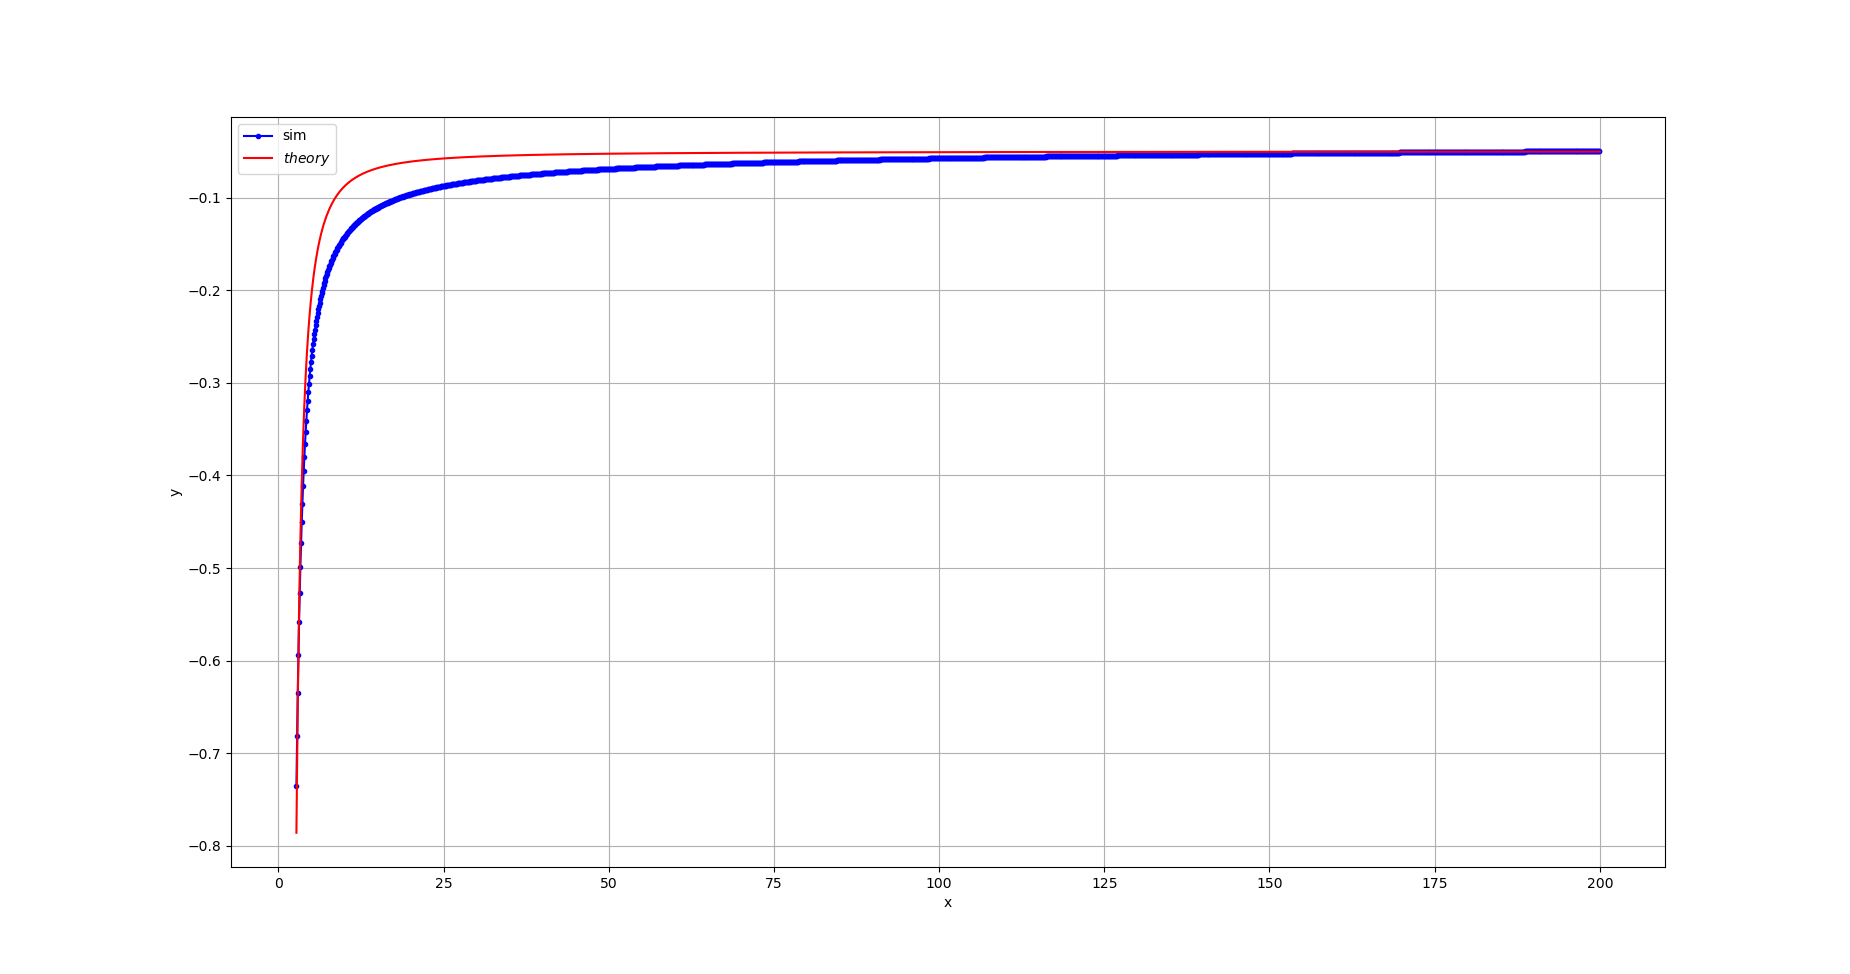
\includegraphics[width=\columnwidth]{figs/Figure_1.png}
	\label{stemplot}
\end{figure}	

\end{document}
